\chapter{Image analysis}

% ROI
% SUV
% Kinetic modeling

In principle, PET and SPECT have the potential to provide quantitative images,
that is pixel values can be expressed in Bq/ml. This is only possible if the
reconstruction is based on a ``sufficiently accurate'' model, e.g. if
attenuation is not taken into account, the images are definitely not
quantitative. It is difficult to define ``sufficiently accurate'', the
definition should certainly depend upon the application. Requirements for
visual inspection are different from those for quantitative analysis.

In image analysis often {\em regions of interest} (ROI's) are used. A region
of interest is a set of pixels which are supposed to belong together. Usually,
an ROI is selected such that it groups pixels with (nearly) identical
behavior, e.g. because they belong to the same part of the same organ. The
pixels are grouped because the relative noise on the mean value of the ROI is
lower than that on the individual pixels, so averaging over pixels results in
strong noise suppression. ROI definition must be done carefully, since
averaging over non-homogeneous regions leads to errors and artifacts! Ideally
an ROI should be three-dimensional. However, mostly two dimensional ROI's
defined in a single plane are used for practical reasons (manual ROI
definition or two-dimensional image analysis software).

In this chapter only two methods of quantitative analysis will be
discussed: standard uptake values (SUV) and the use of compartmental
models. SUV's are simple to compute, which is an important advantage
when the method has to be used routinely. In contrast, tracer kinetic
analysis with compartmental models is often very time consuming, but
it provides more quantitative information.  In nuclear medicine it is
common practice to study the kinetic behavior of the tracer, and many
more analysis techniques exist. However, compartmental modeling is
among the more complex ones, so if you understand that technique,
learning the other techniques should not be too difficult.  The book
by Cherry, Sorenson and Phelps \cite{Cherry} contains an excellent
chapter on kinetic modeling and discusses several analysis techniques.


\section{Standardized Uptake Value}
%%%%%%%%%%%%%%%%%%%%%%%%%%%%%%%%%%%
The standardized uptake value provides a robust scale of tracer amounts. It is
defined as:
\begin{eqnarray}
  \mbox{SUV}_j & = & \frac{\mbox{tracer concentration in $j$}}
                          {\mbox{average tracer concentration}}\\
  & = & \frac{\mbox{tracer amount in Bq/g at pixel $j$}}
                      {\mbox{total dose in Bq / total mass in g}}
\end{eqnarray}
To compute it, we must know the total dose administered to the patient. Since
the total dose is measured prior to injection, and the image is produced after
injection, we must correct for the decay of the tracer in between. Moreover,
the tracer amounts are measured with different devices: the regional tracer
concentration is measured with the SPECT or PET, the dose is measured with a
radionuclide calibrator. Therefor, the sensitivity of the tomograph must be
determined. This is done by acquiring an image of a uniform phantom filled
with a know tracer concentration. From the reconstructed phantom image we can
compute a calibration factor which converts ``reconstructed pixel values''
into Bq/ml (see section \ref{sec:scalefactor}).

A SUV of 1 means that the tracer concentration in the ROI is identical
to the average tracer concentration in the entire patient body. A SUV
of 4 indicates markedly increased tracer uptake. The SUV-value is
intended to be robust, independent from the administered tracer amount
and the mass of the patient. However, it changes with time, since the
tracer participates in a metabolic process. So SUVs can only be
compared if they correspond to the same time after injection. Even
then, one can think of many reasons why SUV may not be very
reproducible, and several publications have been written about its
limitations.  Nevertheless, it works well in practice and is used all
the time.

The SUV is a way to quantify the tracer concentration. But we don't really
want to know that. The tracer was injected to study a metabolic process, so
what we really want to quantify is the intensity of that process. The next
section explains how this can be done. Many tracers have been designed to
accumulate as a result of the metabolic process being studied. If the tracer
is accumulated to high concentrations, many photons will be emitted resulting
in a signal with good signal to noise ratio. In addition, although the tracer
concentration is not nicely proportional to the metabolic activity, it is
often an increasing function of that activity, so it still provides useful
information.

\section{Tracer kinetic modeling}
%%%%%%%%%%%%%%%%%%%%%%%%%%%%%%%%%%
\subsection{Introduction}
%========================
\begin{figure}[tb]
\centering
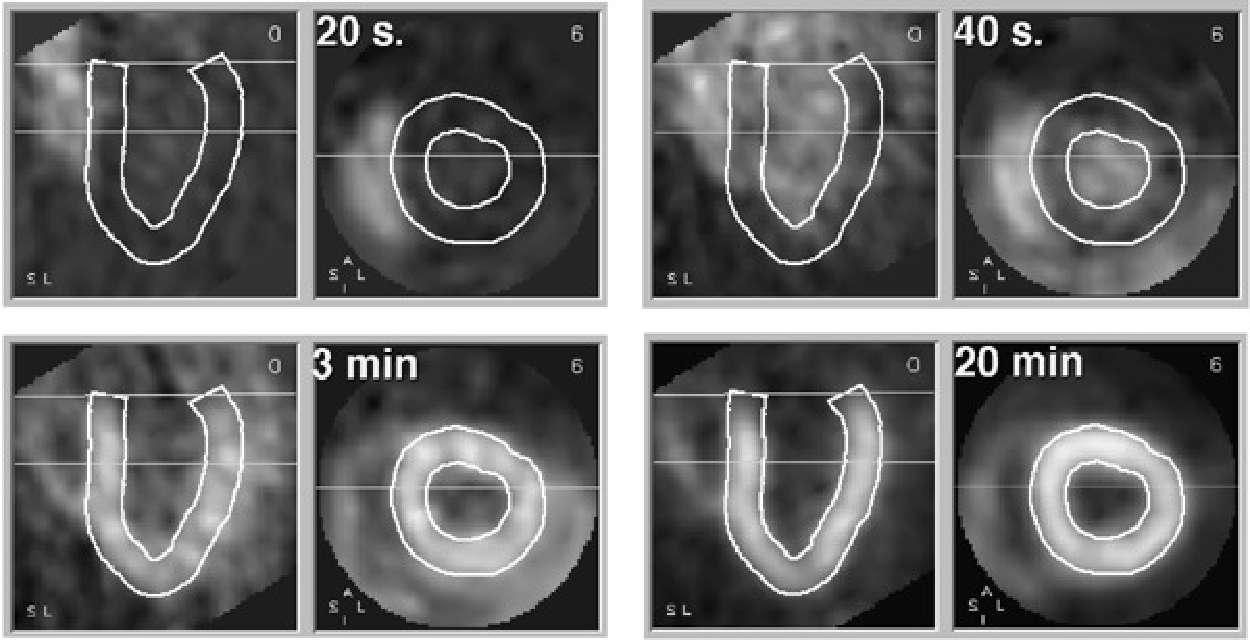
\includegraphics[width=\figbig]{figs/fig_dyncardio.pdf}
\caption{\label{fig:dyncardio} \emph{Four samples from a dynamic
study. Each sample shows a short axis and long axis slice through the
heart. The wall of the left ventricle is delineated. 20 s after
injection, the tracer is in the right ventricle. At 40 s it arrives in
the left ventricle. At 3 min, the tracer is accumulating in the
ventricular wall. At 20 min, the tracer concentration in the wall is
increased, resulting in better image quality.}}
\end{figure}

The evolution of the tracer concentration as a function of time can be
imaged with PET (or SPECT) using ``dynamic acquisition''. Instead of
creating a single image, a series of images is created, typically
starting at the time of tracer injection and continuing for 30 - 90
minutes, depending on the tracer and the kinetic model that is used to
analyse the results.

The evolution of the tracer concentration with time in a particular
point (pixel) depends on the tracer and on the characteristics of the
tissue in that point. Figure \ref{fig:dyncardio} shows the evolution
of radioactive ammonia $^{13}$NH$_3$ (recall that $^{13}$N is a
positron emitter) in the heart region. This is a perfusion tracer: its
concentration in tissue depends mainly on blood delivery to the
cells. The tracer is injected intravenously, so it first shows up in
the right atrium and ventricle. From there it goes to the lungs, and
arrives in the left ventricle after another 20 s. After that, the
tracer is gradually removed from the blood since it is accumulated in
tissue. The myocardial wall is strongly perfused, after 20 min
accumulation in the left ventricular wall is very high, and even the
thin right ventricular wall is clearly visible.

The most important factor determining the dynamic behavior of ammonia
is blood flow. However, the ammonia concentration is not {\em
proportional} to blood flow. To quantify the blood flow in ml blood
per g tissue and per s, the flow must be computed from dynamic
behavior of the tracer. To do that, we need a mathematical model that
describes the most important features of the metabolism for this
particular tracer. Since different tracers trace different metabolic
processes, different models may be required for different tracer.

\subsection{The compartmental model}
%===================================
\subsubsection{The compartments}
%-------------------------------
In this section, the three compartment model is described. It is a
relatively general model and can be used for a few different
tracers. We will focus on the tracer $^{18}$F-fluorodeoxyglucose
(FDG), which is a glucose analog.  ``Analog'' means that it is {\em
no} glucose, but that it is sufficiently similar to follow, to some
extent, the same metabolic pathway as glucose. In fact, it is a better
tracer than radioactive glucose, because it is trapped in the cell,
while glucose is not. When glucose enters the cell, it is metabolized
and the metabolites may escape from the cell. As a result, radioactive
glucose will never give a strong signal. In contrast, FDG is not
completely metabolized (because of the missing oxide), and the
radioactive $^{18}$F atom stays in the cell. If the cells have a high
metabolism, a lot of tracer will get accumulated resulting in a strong
signal (many photons will be emitted from such a region, so the signal
to noise ratio in the reconstructed image will be good).

\begin{figure}[tb]
\centering
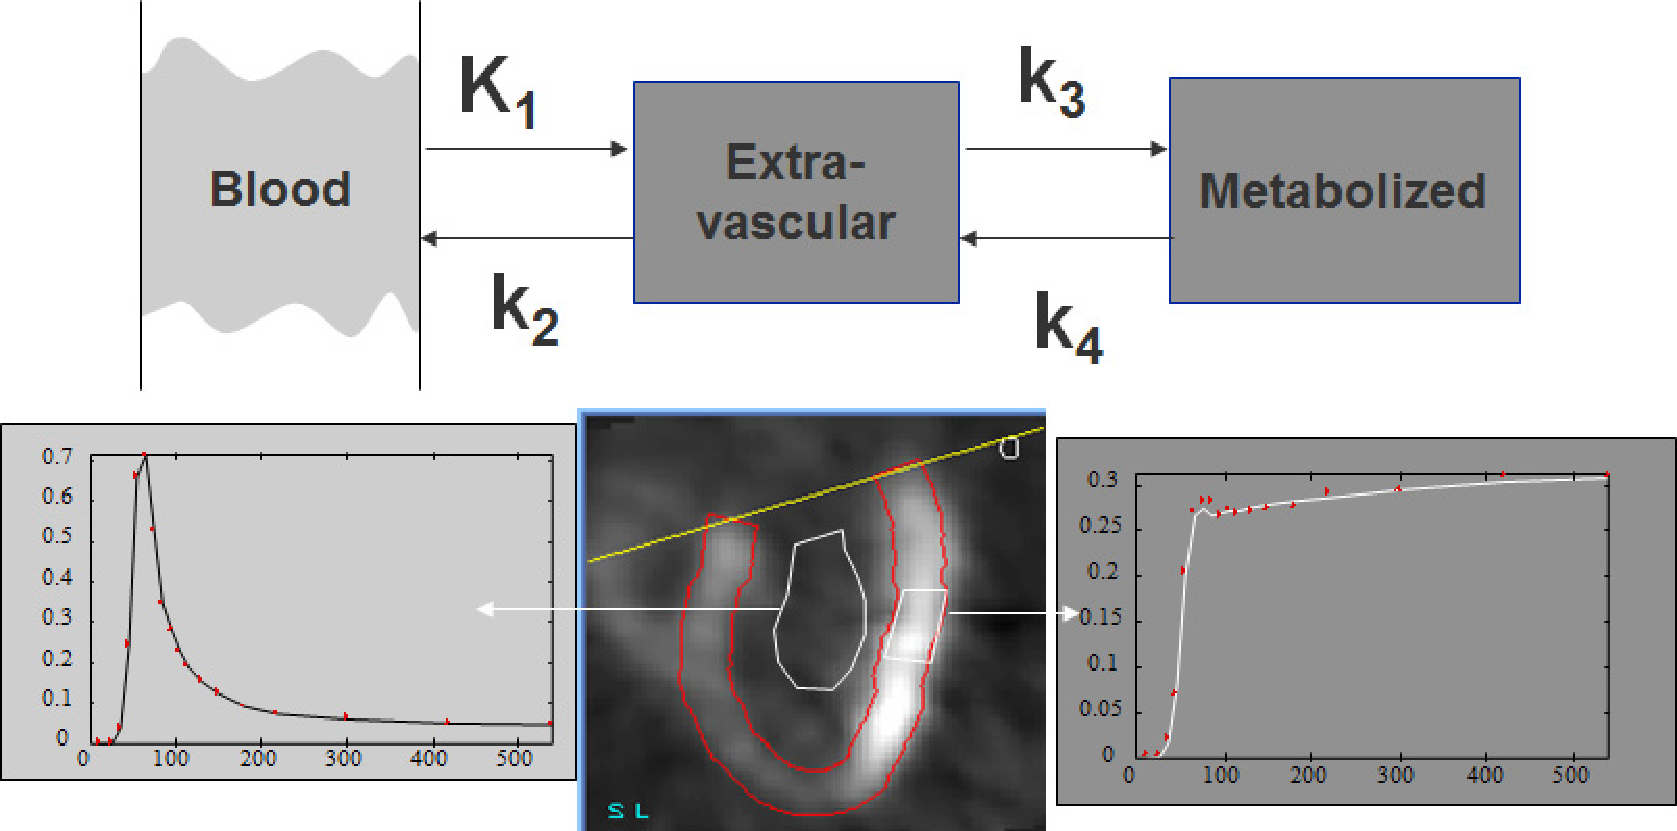
\includegraphics[width=\figbig]{figs/fig_kinemodel.pdf}
\caption{\label{fig:kinemodel} \emph{Three compartment model, and
corresponding regions in a cardiac study. The first compartment represents
plasma concentration (blood pool ROI), the second and third compartment
represent the extavascular tracer in original and metabolized form (tissue
ROI). For the tissue curve, both the measured points and the fitted curve are
shown.}}
\end{figure}

Figure \ref{fig:kinemodel} shows the three compartmental model and its
relation to the measured concentrations. The first compartment represents the
radioactive tracer molecule present in blood plasma. The second compartment
represents the unmetabolized tracer in the ``extravascular space'', that is,
everywhere except in the blood. The third compartment represents the
radioactive isotope after metabolization (so it may now be part of a very
different molecule). In some cases, the compartments correspond nicely to
different structures, but in other cases the compartments are
abstractions. E.g., the second two compartments may be present in a single
cell. We will denote the blood plasma compartment with index {\bf P}, the
extravascular compartment with index {\bf E} and the third compartment with
index {\bf M}.

These compartments are an acceptable simplified model for the different stages
in the FDG and glucose pathways. A model for another tracer may need fewer or
more compartments.

To analyse the tracer concentration curves with the compartmental
model, regions of interest (ROI) are drawn in the image and the mean
tracer concentration in the ROI as a function of time is extracted to
produce the time-activity curves. In figure \ref{fig:kinemodel} a
region is drawn inside the left ventricle to obtain the tracer
concentration in the blood. A second region is drawn in the left
ventricular wall to obtain the tracer concentration in that region of
the heart. The model is then applied to analyse how the concentration
in the blood influences the concentration in the tissue.
%
\begin{figure}[tb]
\centering
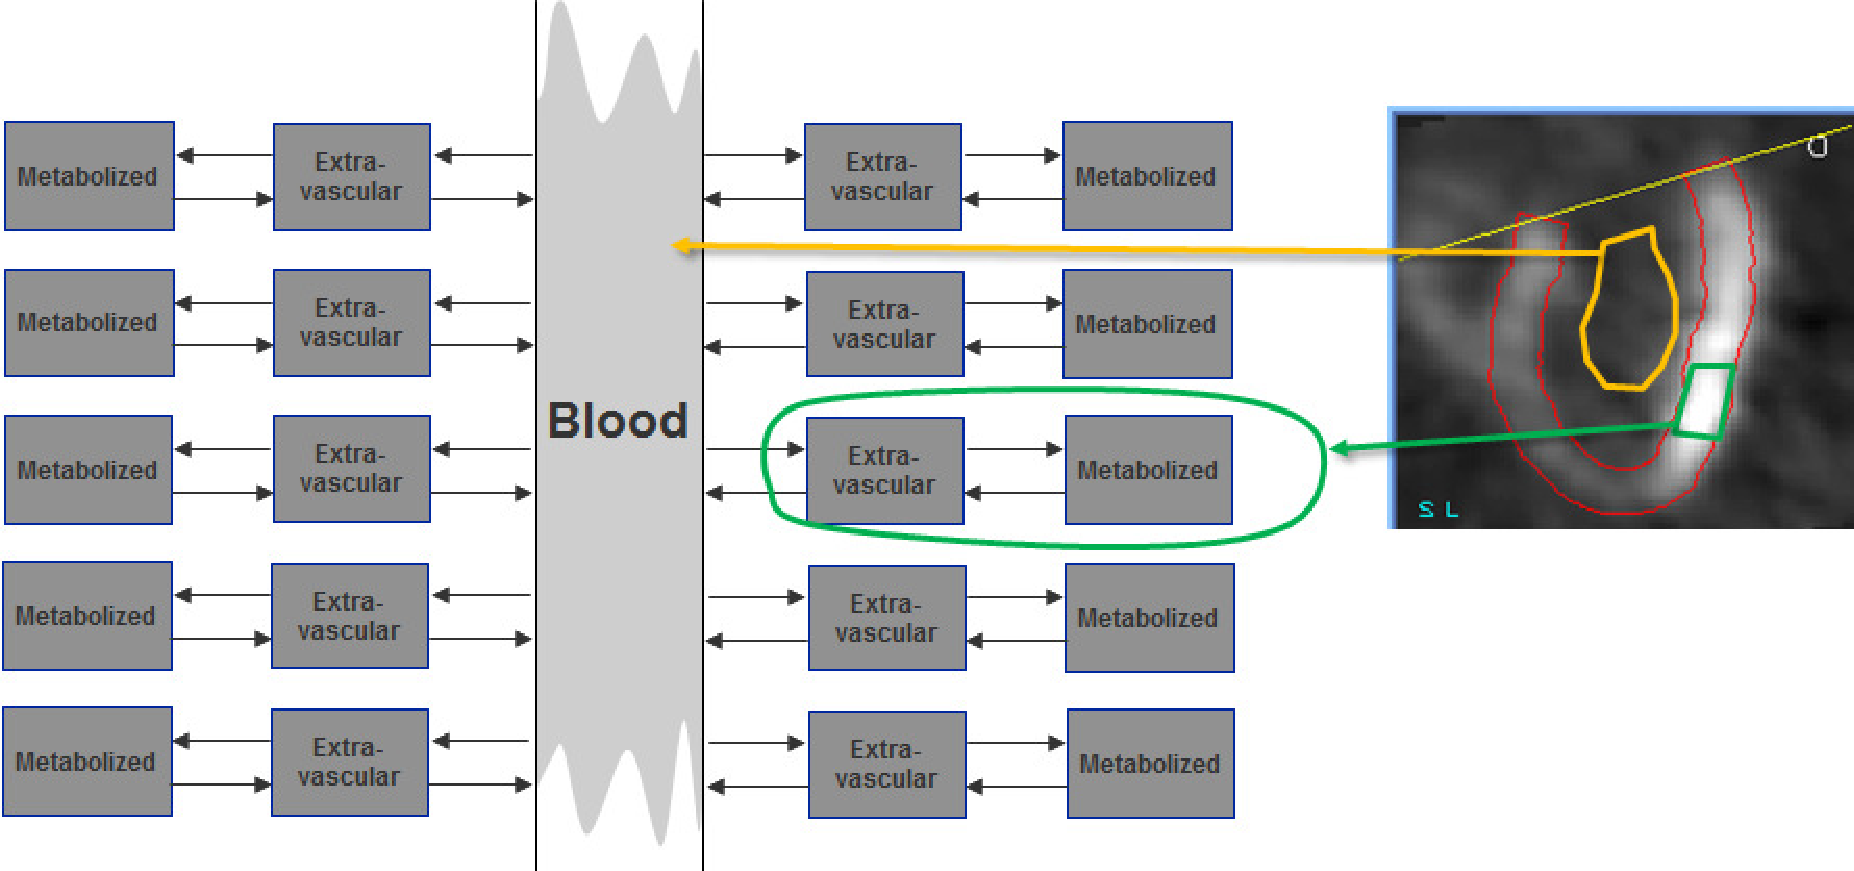
\includegraphics[width=\figbig]{figs/fig_kinemodel2.pdf}
\caption{\label{fig:kinemodel2} \emph{The time-dependent tracer
    concentration in the blood and the rate constants in the tissue
    region determine the evolution of the tissue tracer
    concentration. The blood interacts with a large amount of
    tissue. Since the tissue region we study is small, its effect on
    the blood concentration is negligible.}}
\end{figure}
%
As illustrated in figure \ref{fig:kinemodel2}, the analysis must
explain how the tissue concentration is determined by the blood
concentration and the tissue features. In contrast, the blood
concentration is essentially independent of the concentration in the
region we study. It is determined by the way the tracer is injected
and by the tracer exchange with the entire body. The contribution of
the small region we study to the blood concentration is negligible
compared to the contribution of the entire body.

\subsubsection{The rate constants}
%---------------------------------
The amount of tracer in a compartment can be specified in several ways: number
of molecules, mole, gram or Bq. All these numbers are directly proportional to
the absolute number of molecules. If we study a single gram of tissue, the
amounts can be expressed in Bq/g, which is the unit of concentration. Remark,
though, that these are not tracer concentrations of the compartments, since the
gram tissue contains several compartments.

The compartments may exchange tracer molecules with other compartments. It is
assumed that this exchange can be described with simple first order rate
constants. This means that the amount of tracer traveling away from a
compartment is proportional to the amount of tracer in that compartment. The
constant of proportionality is called a {\em rate constant}. For the three
compartment model, there are two different types of rate constants. Constant
$K_1$ is a bit different from $k_2$, $k_3$ and $k_4$ because the first
compartment is a bit different from the other two  (fig. \ref{fig:kinemodel}).

The amount of tracer going from the blood plasma compartment to the
extravascular compartment is
\begin{equation}
  \mbox{Tracer}_{P \rightarrow E} = K_1 C_P
\end{equation}
where $C_P$ is the plasma tracer concentration (units: Bq/ml). $K_1$ is the
product of two factors. The first one is the blood flow $F$, the amount of
blood supplied in every second to the gram tissue. $F$ has units ml/(s g).
The second factor is the extraction fraction $f$, which specifies which
fraction of the tracer passing by in $P$ is exchanged with the second
compartment $E$. Since it is a fraction, $f$ has no unit. For some tracers,
$f$ is almost 1 (e.g. for radioactive water). For other tracers it is 0, which
means that the tracer stays in the blood. For FDG it is in
between. Consequently, the product $K_1 C_P = F f C_P$ has units Bq/(s g) and
tells how many Bq are extracted from the blood per second and per gram tissue.
$C_P$ is a function of the time, $K_1$ is not (or more precisely, we assume
it stays constant during the scan). Both $K_1$ and $C_P$ are also a
function of position: the situation will be different in different tissue types.

The amount of tracer going from $E$ to $M$ equals:
\begin{equation}
  \mbox{Tracer}_{E \rightarrow M} = k_3 C_E(t),
\end{equation}
where $C_E$ is the total amount of tracer in compartment $E$ per gram tissue
(units: Bq/g). Constant $k_3$ tells which fraction of the available tracer is
metabolized in every second, so the unit of $k_3$ is 1/s. The physical meaning
of $k_2$ and $k_4$ is similar: they specify the fractional transfer per
second.

\subsubsection{The target molecule}
%----------------------------------
The tracer is injected to study the metabolism of a particular molecule. It is
assumed that the metabolic process being studied is constant during the
measurement, and that the target molecule (glucose in our example) has reached
a steady state situation. Steady state means that a dynamic equilibrium has
been reached: all concentrations remain constant. Steady state can only be
reached with well-designed feedback systems (poor feedback systems oscillate),
but it is reasonable to assume that this is the case for metabolic processes
in living creatures.

Since FDG and glucose are not identical, their rate constants are not
identical.  The glucose rate constants will be labeled with the letter
$g$. The glucose and FDG amounts are definitely different: glucose is
abundantly present and is in steady state condition. FDG is present in
extremely low concentrations (pmol) and has not reached steady state since the
images are acquired immediately after injection.

The plasma concentration $C_P^g$ is supposed to be constant. We can
measure it by determining the glucose concentration in the plasma from
a venous blood sample. The extravascular glucose amount $C_E^g$ is
supposed to be constant as well, so the input must equal the
output. For glucose, $k_4^g$ is very small. Indeed, $k_4^g$
corresponds to reversal of the initiated metabolization, which happens
only rarely. Setting $k_4^g$ to zero we have
\begin{equation}
\frac{d C_E^g}{dt} = 0 = K_1^g C_P^g - (k_2^g + k_3^g) C_E^g.
\end{equation}
Thus, we can compute the unknown glucose amount $C_E^g$ from the known plasma
concentration $C_P^g$:
\begin{equation}
  C_E^g = \frac{K_1^g}{k_2^g + k_3^g} C_P^g.
\end{equation}
The glucose metabolization in compartment $M$ is proportional to the glucose
transport from $E$ to $M$. Of course, the glucose metabolites may be
transported back to the blood, but we don't care. We are only interested in
glucose. Since it ceases to exist after transport to compartment $M$ we ignore
all further steps in the metabolic pathway. In our compartment model, it is as
if glucose is accumulated in the metabolites compartment. This virtual
accumulation rate is the metabolization rate we want to find:
\begin{eqnarray}
  \frac{d C_M^g}{d t} = k_3^g C_E^g & = & 
   \frac{K_1^g k_3^g}{k_2^g + k_3^g} C_P^g.\\
  & = & \bar{K^g}  C_P^g. \hspace{2cm} \mbox{$($definition of } \bar{K^g})
\end{eqnarray}

So if we can find the values of the rate constants, we can compute the glucose
metabolization rate. As mentioned before, we cannot compute them via the
tracer, since it has different rate constants. However, it can be shown that,
due to its similarity, the trapping of FDG is {\em proportional} to the glucose
metabolic rate. The constant of proportionality depends on the tissue type
(difference in affinity for both molecules), but not on the tracer
concentration. The constant of proportionality is usually called ``the lumped
constant'', because careful theoretical analysis shows that it is a combination
of several constants. So the lumped constant LC is:
\begin{equation}
  LC = \frac{\frac{K_1 k_3}{k_2 + k_3}}{\frac{K_1^g k_3^g}{k_2^g + k_3^g}}
  = \frac{\bar{K}}{\bar{K^g}}
\end{equation}
For the (human) brain (which gets almost all its energy from glucose)
and for some other organs, several authors have attempted to measure
the lumped constant. The values obtained for brain are around
0.8. This means that the human brain has a slight preference for
glucose: if the glucose and FDG concentrations in the blood would be
identical, the brain would accumulate only 8 FDG molecules for every
10 glucose molecules. If we had used radioactive glucose instead of
deoxyglucose, the tracer and target molecules would have had identical
rate constants and the lumped constant would have been 1. But as
mentioned before, with glucose as a tracer, the radioactivity would
not accumulate in the cells, which would result in poorer PET images.

\subsubsection{The tracer}
%-------------------------
\paragraph{Problem statement\\}
%''''''''''''''''''''''''''''''
Because the lumped constant is known, we can compute the glucose
metabolization rate from the FDG trapping rate. To compute the trapping rate,
we must know the FDG rate constants. Since the tracer is not in steady state,
the equations will be a bit more difficult than for the target molecule.  We
can easily derive differential equations for the concentration changes in the
second and third compartment:
\begin{eqnarray}
  \frac{dC_E(t)}{dt} & = & K_1 C_P(t) - (k_2 + k_3) C_E(t) \label{eq:C_E}\\
  \frac{dC_M(t)}{dt} & = & k_3 C_E(t) \label{eq:C_M}
\end{eqnarray}
For a cardiac study, we can derive the tracer concentration $C_P(t)$ in the
blood from the pixel values in the center of the left ventricle or atrium. If
the heart is not in the field of view, we can still determine $C_P(t)$ by
measuring the tracer concentrations in blood samples withdrawn at regular time
intervals.  As with the SUV computations, this requires cross-calibration of
the plasma counter to the PET camera.

The compartments $E$ and $M$ can only be separated with subcellular
resolution, so the PET always measures the sum of both amounts, which we will
call $C_I(t)$:
\begin{equation}
  C_I(t) = C_E(t) + C_M(t).
\end{equation}

Consequently, we must combine the equations (\ref{eq:C_E}) and (\ref{eq:C_M})
in order to write $C_I(t)$ as a function of $C_P(t)$ and the rate
constants. This is the operational function. Since $C_I(t)$ and $C_P(t)$ are
known, the only remaining unknown variables will be the rate constants, which
are obtained by solving the operational function.

\paragraph{Deriving the operational function\\}
%''''''''''''''''''''''''''''''''''''''''''''
To deal with differential equations, the Laplace transform is a valuable
tool. Appendix \ref{app:laplace} gives the definition and a short table of the
features we need for the problem at hand. The strength of the Laplace
transform is that derivatives and integrals with respect to $t$ become simple
functions of $s$. After transformation, elimination of variables is easy. The
result is then back-transformed to the time domain.  Laplace transform of
(\ref{eq:C_E}) and (\ref{eq:C_M}) results in
\begin{eqnarray}
  s c_E(s) & = & K_1 c_P(s) - (k_2 + k_3) c_E(s) \label{eq:sc_E}\\
  s c_M(s) & = & k_3 c_E(s)  \label{eq:sc_M}
\end{eqnarray}
where we have assumed that at time $t=0$ (time of injection) all tracer
amounts are zero.  From (\ref{eq:sc_E}) we find $c_E(s)$ as a function of
$c_P(s)$. Inserting in (\ref{eq:sc_M}) produces $c_M(s)$ as a function of
$c_P(s)$.
\begin{eqnarray}
  c_E(s) & = & \frac{K_1}{s + k_2 + k_3} c_P(s)\\
  c_M(s) & = & \frac{K_1 k_3}{s (s + k_2 + k_3)} c_P(s)\\
  c_I(s) & = & c_E(s) + c_M(s) \\
         & = & \left( \frac{K_1}{s + k_2 + k_3} 
                    + \frac{K_1 k_3}{s (s + k_2 + k_3)}\right) c_P(s)
           \label{eq:c_I}
\end{eqnarray}
The two factors in $s$ can be split from the denominator using the equation
\begin{equation}
  \frac{a}{x(x + b)} = \frac{a}{b} \left( \frac{1}{x} - \frac{1}{x+b} \right)
\end{equation}
Applying this to (\ref{eq:c_I}) and rearranging a bit yields:
\begin{equation}
  c_I(s) = \frac{K_1 k_2}{(k_2 + k_3)} \frac{c_P(s)}{(s + k_2 + k_3)} + 
           \frac{K_1 k_3}{(k_2 + k_3)} \frac{c_P(s)}{s}
\end{equation}
Applying the inverse Laplace transform is now straightforward (see appendix
\ref{app:laplace}) and produces the operational function:
\begin{equation}
  C_I(t) = \frac{K_1 k_2}{k_2 + k_3} \int_0^t C_P(u) e^{-(k_2 + k_3)(t - u)}du
         + \frac{K_1 k_3}{k_2 + k_3} \int_0^t C_P(u) du. \label{eq:3comp_ci}
\end{equation}

\begin{figure}[tb]
\centering
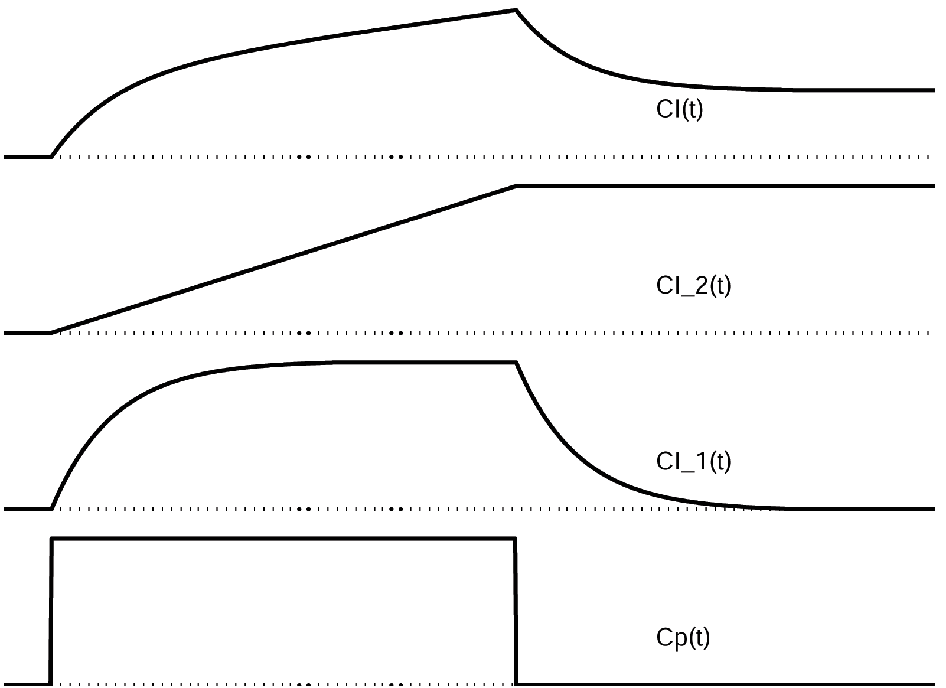
\includegraphics[width=\figone]{figs/fig_3comp_ci.pdf}
\caption{\label{fig:3comp_ci} \emph{The tracer amount $C_I(t)$ and its two
terms when $C_P(t)$ is a step function (equation (\ref{eq:3comp_ci})).}}
\end{figure}
%
Figure \ref{fig:3comp_ci} plots $C_I$ and the two terms of equation
(\ref{eq:3comp_ci}) for the case when $C_P(t)$ is a step function. $C_P(t)$ is
never a step function, but the plot provides interesting information. The
first term of (\ref{eq:3comp_ci}) represents tracer molecules that leave the
vascular space, stay a while in compartment $E$ and then return back to the
blood. As soon as the tracer is present in the blood, this component starts to
grow until it reaches a maximum. When $C_P(t)$ becomes zero again, the
component gradually decreases towards zero. This first term follows the input,
but with some delay (CI$_1$(t) in fig. \ref{fig:3comp_ci}).

The second term of (\ref{eq:3comp_ci}) represent tracer molecules that
enter compartment $E$ and will never leave (CI$_2$(t) in
fig. \ref{fig:3comp_ci}). Eventually, they will be trapped in
compartment $M$. Note that the first term is not equal to but smaller
than $C_E(t)$. The reason is that part of the molecules in $E$ will
not return to the blood but end up in $M$. It is easy to compute which
fraction of $C_E(t)$ is described by the first term of
(\ref{eq:3comp_ci}). (The rest of $C_E(t)$ and $C_M(t)$ correspond to
the second term of (\ref{eq:3comp_ci}).) This is left as an exercise
to the reader.

\paragraph{Impulse response\\}
%'''''''''''''''''''''''''''''
Equation \ref{eq:3comp_ci} can be rewritten as
\begin{equation}
  C_I(t) = \frac{K_1}{k_2 + k_3} \int_0^t C_P(u) \left(
       k_2 \; e^{-(k_2 + k_3)(t - u)} + k_3 \right) du.
\end{equation}
This is a convolution of the input function with the factor in
brackets, showing that that factor is the impulse response
function. To illustrate this, we simply compute the response to an
impulse, by replacing $C_p(u)$ with a Dirac impulse at time $\xi$:
\begin{eqnarray}
  C_I(t) &=& \frac{K_1}{k_2 + k_3} \int_0^t \delta(u-\xi) \left(
                k_2 \; e^{-(k_2 + k_3)(t - u)} + k_3 \right) du\\
   &=& \frac{K_1}{k_2 + k_3} \left( k_2 \; e^{-(k_2 + k_3)(t - \xi)} +
                k_3 \right).
\end{eqnarray}


\paragraph{Alternative derivation, avoiding the Laplace transform\\}
%'''''''''''''''''''''''''''''''''''''''''''''''''''''''''''''''''
The same result (\ref{eq:3comp_ci}) can be obtained with the method of
variation of parameters.
For simplicity, we set $\beta = k_2 + k_3$,
rewriting equation (\ref{eq:C_E}) as follows
\begin{equation}
   \frac{dC_E(t)}{dt}  =  K_1 C_P(t) - \beta C_E(t). \label{eq:vp1}
\end{equation}
First, we solve the corresponding homogeneous equation, obtained by
dropping the terms independent of $C_E(t)$:
\begin{equation}
   \frac{dC_E(t)}{dt}  =  - \beta C_E(t).
\end{equation}
The solution is $C_E(t) = A e^{-\beta t}$. Now we assume that the
solution to (\ref{eq:vp1}) is similar, except that the constant $A$
must be replaced by a function of $t$: $C_E(t) = A(t) \; e^{-\beta
t}$. Inserting this in (\ref{eq:vp1}) we obtain:
\begin{eqnarray}
   \frac{d ( A(t) \; e^{-\beta t})}{dt} 
             &=&  K_1 C_P(t) - \beta A(t) \; e^{-\beta t}\\
 = \hspace{5mm} 
   \frac{d A(t)}{dt} \; e^{-\beta t} - \beta A(t) e^{-\beta t} 
              &=& K_1 C_P(t) - \beta A(t) \; e^{-\beta t}\\
\Leftrightarrow  \hspace{5mm} 
   \frac{d A(t)}{dt} \; e^{-\beta t} &=& K_1 C_P(t)\\
\Leftrightarrow  \hspace{5mm} 
   A(t) &=& K_1 \int_0^t C_P(u) e^{\beta u} du\\
\Leftrightarrow  \hspace{5mm} 
   C_E(t) = A(t)  \; e^{-\beta t}
      &=& K_1 \int_0^t C_P(u) e^{- \beta (t -u)} du \label{eq:vp2}
\end{eqnarray}
%
Having solved the equation for the first tissue compartment, we can
use $C_E(t)$ to find the activity in the second compartment.  We
simply insert (\ref{eq:vp2}) in the equation (\ref{eq:C_M}) for
$C_M(t)$ to obtain:
\begin{eqnarray}
  \frac{d C_M(t)}{dt} = k_3 C_E(t) 
    &=& K_1 k_3 \int_0^t C_P(u) e^{- \beta (t -u)} du \nonumber\\
    &=& K_1 k_3 \; e^{- \beta t} \; \int_0^t C_P(u) e^{\beta u} du
\end{eqnarray}
and therefore
\begin{equation}
  C_M(t) = K_1 k_3 \; \int_0^t d\xi \; e^{-\beta \xi} 
       \int_0^\xi  C_P(u) e^{\beta u} du.   \label{eq:vp3}
\end{equation}
This is the integral of an integral, which may seem somewhat
intimidating at first. However, it can be simplified using integration
by parts. If you are unfamiliar with that trick, you can easily derive
it by noting that the integral of the derivative of the product of two
functions $f(t)$ and $g(t)$ equals:
\begin{eqnarray}
  f(t) g(t) - f(0) g(0) = \int_0^t \frac{d ((f(\xi) g(\xi))}{d\xi} d\xi
 = \int_0^t \frac{d f(\xi)}{d\xi} g(\xi) d\xi 
   +  \int_0^t f(\xi) \frac{d g(\xi)}{d\xi} d\xi
\end{eqnarray}
And therefore we can write
\begin{equation}
  \int_0^t \frac{d f(\xi)}{d\xi} g(\xi) d\xi = f(t) g(t) - f(0) g(0)
        - \int_0^t f(\xi) \frac{d g(\xi)}{d\xi} d\xi \label{eq:vptrick}
\end{equation}
We apply this trick to get rid of the inner integral in (\ref{eq:vp3})
as follows:
\begin{eqnarray}
  f(\xi) &=& -\frac{e^{-\beta \xi}}{\beta}\\
  \frac{d f(\xi)}{d\xi} &=& e^{-\beta\xi}\\
  g(\xi) &=& \int_0^\xi  C_P(u) e^{\beta u} du\\
  \frac{d g(\xi)}{d\xi} &=& C_P(\xi) e^{\beta \xi}
\end{eqnarray}
With these definitions, the left hand side of (\ref{eq:vptrick}) is
equal to (\ref{eq:vp3}). Note that $g(0) = 0$ here, which makes things
slightly simpler.  The trick converts (\ref{eq:vp3}) into:
\begin{eqnarray}
 C_M(t) &=& K_1 k_3 \left( 
  -\frac{e^{-\beta t}}{\beta} \int_0^t  C_P(u) e^{\beta u} du
  - \int_0^t (-\frac{e^{-\beta u}}{\beta}) C_P(u) e^{\beta u} du
   \right) \nonumber \\
 &=& \frac{K_1 k_3}{k_2 + k_3} \left(
   - \int_0^t C_P(u) e^{-(k_2 + k_3) (t -u)} du + \int_0^t C_P(u) du
 \right) \label{eq:vp4}
\end{eqnarray}
where we have replaced $\beta$ again with $k_2 + k_3$.
Finally, to obtain $C_I(t) = C_E(t) + C_M(t)$ we sum (\ref{eq:vp2})
and (\ref{eq:vp4}):
\begin{eqnarray}
C_I(t) &=& (K_1 - \frac{K_1 k_3}{k_2 + k_3}) 
            \int_0^t C_P(u) e^{- (k_2 + k_3) (t -u)} du \;\;
       + \;\; \frac{K_1 k_3}{k_2 + k_3} \int_0^t C_P(u) du \nonumber\\
 &=&
  \frac{K_1 k_2}{k_2 + k_3} \int_0^t C_P(u) e^{- (k_2 + k_3) (t -u)} du
    \;\; + \;\;
   \frac{K_1 k_3}{k_2 + k_3} \int_0^t C_P(u) du,
\end{eqnarray}
which is identical to equation (\ref{eq:3comp_ci}).

\paragraph{Computing the rate constants with non-linear regression\\}
%'''''''''''''''''''''''''''''''''''''''''
At this point, we have the operational function relating $C_I(t)$ to $C_p(t)$
and the rate constants. We also know $C_p(t)$ and $C_I(t)$, at least in
several sample points (dynamic studies have typically 20 to 40 frames). Every
sample point is an equation, so we actually have a few tens of equations and 3
unknowns. Because of noise and the fact that the operational function is only
an approximation, there is probably no exact solution. The problem is very
similar to the reconstruction problem, which has been solved with the maximum
likelihood approach. The same will be done here. If the likelihood is assumed
to be Gaussian, maximum likelihood becomes weighted least squares.

With this approach, we start with an arbitrary set of rate constants. It is
recommended to start close to the solution if possible, because the likelihood
function may have local maxima. Typically the rate constants obtained in
healthy volunteers are used as a start. With these rate constants and the
known input function $C_p(t)$, we can compute the expected value of
$C_I(t)$. The computed curve will be diff erent from the measured one. Based on
this difference, the non-linear regression algorithm will improve the values
of the rate constants, until the sum of weighted squared differences is
minimal. It is always useful to plot both the measured and computed curves
$C_I(t)$ to verify that the fit has succeeded, since there is small chance
that the solution corresponds to an unacceptable local minimum. In that case,
the process must be repeated, starting from a different set of rate constant
values. The tissue curve in fig.\ \ref{fig:kinemodel} is the result of
non-linear regression. The fit was successful, since the curve is close to the
measured values.

The glucose consumption can now be computed as
\begin{equation}
  \mbox{glucose consumption} =
     \frac{1}{\mbox{LC}} \frac{K_1 k_3}{k_2 + k_3} C_P^g
     = \frac{\bar{K}}{\mbox{LC}} C_P^g \label{eq:glucmet}
\end{equation}

Non-linear regression programs often provide an estimate of the confidence
intervals or standard deviations on the fitted parameters. These can be very
informative. Depending on the shape of the curves, the noise on the data and
the mathematics on the model, the accuracy of the fitted parameters can be
very poor. However, the errors on the parameters are correlated such that the
accuracy on $\bar{K}$ is better than the accuracy on the individual rate
constants. 

\paragraph{Computing the trapping rate with linear regression\\}
%'''''''''''''''''''''''''''''''''''''''''
By introducing a small approximation, the computation of the glucose
consumption can be simplified. Figure \ref{fig:kinemodel} shows a typical
blood function. The last part of the curve is always very smooth. As a result,
the first term of (\ref{eq:3comp_ci}) nicely follows the shape of
$C_p(t)$. Stated otherwise, $C_p(u)$ changes very little over the range where
$e^{-(k_2 + k_3)(t - u)}$ is significantly different from zero. Thus, we can
put $C_p(t)$ in front of the integral sign. Since $t$ is large relative to the
decay time of the exponential, we can set $t$ to $\infty$:
\begin{eqnarray}
\int_0^t C_P(u) e^{-(k_2 + k_3)(t - u)}du
  & \simeq &  C_P(t) \int_0^t  e^{-(k_2 + k_3)(t - u)}du\\
  & =      &  C_P(t) \int_0^t  e^{-(k_2 + k_3)u}du\\
  & \simeq &  C_P(t) \int_0^\infty  e^{-(k_2 + k_3)u}du\\
  & = & \frac{C_p(t)}{k_2 + k_3}
\end{eqnarray}
The operational function then becomes:
\begin{equation}
  C_I(t) \simeq \frac{K_1 k_3}{k_2 + k_3} \int_0^t C_P(u) du + 
  \frac{K_1 k_2}{(k_2 + k_3)^2} C_P(t).
\end{equation}
Now both sides are divided by $C_p(t)$:
\begin{equation}
  \frac{C_I(t)}{C_P(t)} \simeq 
    \frac{K_1 k_3}{k_2 + k_3} \frac{\int_0^t C_P(u) du}{C_P(t)} + 
  \frac{K_1 k_2}{(k_2 + k_3)^2}. \label{eq:patlak}
\end{equation}
Equation (\ref{eq:patlak}) says that $C_I(t)/C_P(t)$ is a linear function of
$\int_0^t C_P(u) du / C_P(t)$, at least for large values of $t$. We can ignore
the constants, all we need is the slope of the straight curve. This can be
obtained with simple linear regression. For linear regression no iterations
are required, there is a closed form expression, so this solution is orders of
magnitudes faster to compute than the previous one. 

The integral $\int_0^t C_P(u) du / C_P(t)$ has the unit of time. If $C_P(t)$
would be a constant, the integral simply equals $t$. It can be regarded as a
correction, required because $C_P(t)$ is not constant but slowly varying. As
shown in figure \ref{fig:3comp_ci}, when $C_P(t)$ is constant, $C_I(t)$ has
a linear and a constant term. Equation (\ref{eq:3comp_ci}) confirms that the
slope of the linear term is indeed $\bar{K}$. A potential disadvantage is that
the values of the rate constants are not computed.


\section{Image quality}
%======================
It is extremely difficult to give a useful definition of image quality. As a
result, it is even more difficult to measure it. Consequently, often debatable
measures of image quality are being used. This is probably unavoidable, but it
is good to be fully aware about the limitations.

\subsection{Subjective evaluation}
%---------------------------------
A very bad but very popular way to assess the performance of some new method
is to display the image produced by the new method together with the image
produced in the classical way, and see if the new image is ``better''. In many
cases, you cannot see if it is better. You can see that you like it better for
some reason, but that does not guarantee that it will lead to an improvement
in the process (e.g. making a diagnosis) to which the image is supposed to
contribute.

As an example, a study has been carried out to determine the effect of
2D versus 3D PET imaging on the diagnosis of a particular disease, and
for a particular PET system. In addition, the physicians were asked to
tell what images they preferred. The physicians preferred the 3D
images because they look nicer, but their diagnosis was statistically
significantly better on the 2D images (because scatter contribution
was lower).

It is not forbidden to look at an image (in fact, it is usually a good
idea to look at it carefully), but it is important not to jump to a
conclusion.

\subsection{Task dependent evaluation}
%-------------------------------------
The best way to find out if an image is good, is to use it as planned and
check if the results are good. Consequently, if a new image generation or
processing technique is introduced, it has to be compared very carefully to
the classical method on a number of clinical cases. Evaluation must be done
blindly: if the observer remembers the image from the first method when
scoring the image from the second method, the score is no longer objective. If
possible the observer should not even be aware of the method, in order to
exclude the influence of possible prejudice about the methods.

\subsection{Continuous and digital}
%----------------------------------
Intuitively, the best image is the one closest to the truth. But in emission
tomography, the truth is a continuous tracer distribution, while the image is
digital. It is not always straightforward to define how a portion of a
continuous curve can be best approximated as a single value. The problem
becomes particularly difficult if the images to be compared use a different
sampling grid (shifted points or different sampling density). So if possible,
make sure that the sampling is identical.

\subsection{Bias and variance}
%-----------------------------
Assume that we have a reference image e.g. in a simulation experiment. In
this case, we know the true image, and in most cases it is even digital. Then
we can compare the difference between the true image and the image to be
evaluated. A popular approach is to compute the mean squared difference:
\begin{equation}
  \mbox{mean squared difference} = \frac{1}{J} \sum_{j=1}^J (\lambda_j - r_j)^2,
\end{equation}
where $\lambda_j$ and $r_j$ are the image and the reference image
respectively.  This approach has two problems. First, it assumes that
all pixels are equally important, which is almost never true. Second,
it combines systematic (bias) and random (variance) deviations. It is
better to separate the two, because they behave very differently. This
is illustrated in figure \ref{fig:bias_var}. Suppose that a block wave
was measured with two different methods A and B, producing the noisy
curves shown at the top row. Measurement A is noisier, and its sum of
squared differences with the true wave is twice as large as that of
measurement B. If we know that we are measuring a block wave, we know
that a bit of smoothing is probably useful. The bottom row shows the
result of smoothing. Now measurement A is clearly superior. The reason
is that the error in the measurement contains both bias and
variance. Smoothing reduces the variance, but increases the bias. In
this example the true wave is smooth, so variance is strongly reduced
by smoothing, while the bias only increases near the edges of the
wave.  If we keep on smoothing, the entire wave will converge to its
mean value; then there is no variance but huge bias. Bias and variance
of a sample (pixel) $j$ can be defined as follows:
\begin{eqnarray}
  \mbox{bias}_j     & = & E(\lambda_j - r_j)\\
  \mbox{variance}_j & = & E\left((\lambda_j - E(\lambda_j))^2 \right),
\end{eqnarray}
where $E(x)$ is the expectation of $x$. Variance can be directly computed from
repeated independent measurements. If the true data happen to be smooth and if
the measurement has good resolution, neighboring samples can be regarded as
independent measurements. Bias can only be computed if the true value is known.

In many cases, there is the possibility to trade in variance for bias by
smoothing or imposing some constraints. Consequently, if images are compared,
bias and variance must be separated. If an image has better bias for the same
variance, it is probably a ``better'' image. If an image has larger bias and
lower variance when compared to another image, the comparison is meaningless.

\begin{figure}[tb]
\centering
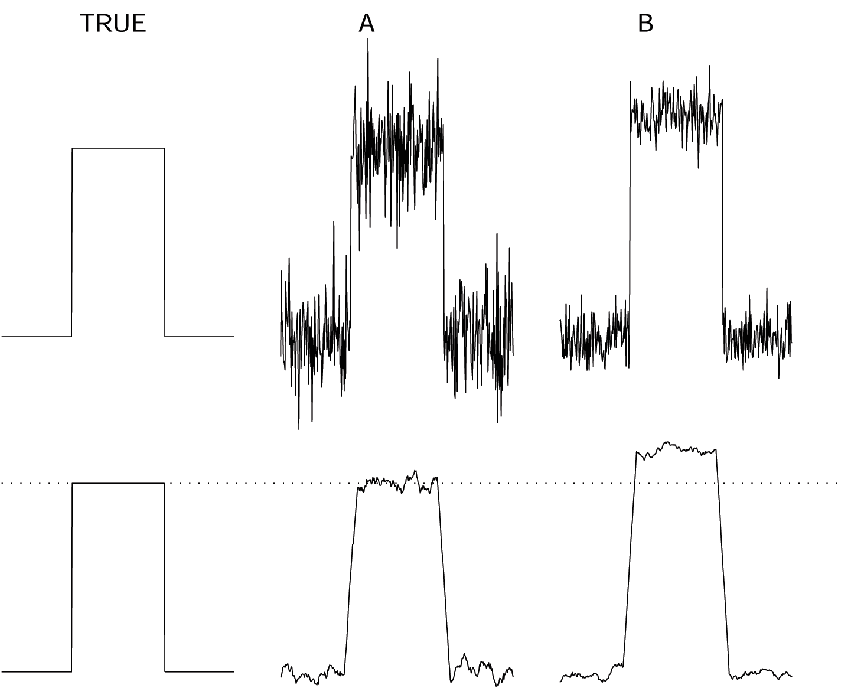
\includegraphics[width=\figone]{figs/fig_bias_var.pdf}
\caption{\label{fig:bias_var} \emph{Top: a simulated true block wave and two
measurements A and B with different noise distributions. Bottom: the true
block wave and the same measurements, smoothed with a simple rectangular
smoothing kernel.}}
\end{figure}

\subsection{Evaluating a new algorithm}
%-----------------------------------
A good way to evaluate a new image processing algorithm (e.g. an algorithm for
image reconstruction, for image segmentation, for registration of images from
different modalities) is to apply the following sequence:
\begin{enumerate}
  \item evaluation on computed, simulated data
  \item evaluation on phantom data
  \item (evaluation on animal experiments)
  \item evaluation on patient data
\end{enumerate}
This sequence is in order of increasing complexity and decreasing
controllability. Tests on patient data are required to show that the method
can be used. However, if such a test fails it is usually very difficult to
find out why. To find the problem, simple and controllable data are required.
Moreover, since the true solution is often not known in the case of patient
data, it is possible that failure of the method remains undetected.
Consequently, there is no gain in trying to skip one or a few stages, and with
a bit of bad luck it can have serious consequences.

Evaluation on simulation has the following important advantages:
\begin{itemize}
  \item The truth is known, comparing the result to the true answer is simple.
        This approach is also very useful for finding bugs in the algorithm or
        its implementation.
  \item Data can be generated in large numbers, sampling a predefined
        distribution. This enables direct quantitative analysis of bias and
        variance.
  \item Complexity can be gradually increased by making the simulations more
        realistic, to analyze the response to various physical phenomena
        (noise, attenuation, scatter, patient motion \ldots).
  \item A nice thing about emission tomography is that it is relatively easy
        to make realistic simulations. In addition, many research groups are
        willing to share simulation code.
  \item It is possible to produce simulations which are sufficiently realistic
        to have them diagnosed by the nuclear medicine physicians. Since the
        correct diagnosis is known, this allows evaluation of the effect of
        the new method on the final diagnosis.
\end{itemize}

When the method survives complex simulations it is time to do phantom
experiments. Phantom experiments are useful because the true system is always
different from even a very realistic simulation. If the simulation phase has
been done carefully, phantom experiments are not likely to cause much trouble.

A possible intermediate stage is the use of animal experiments, which can be
required for the evaluation of very delicate image processing techniques
(e.g. preparing stereotactic operations). Since the animal can be sacrificed,
it is possible, at least to some extent, to figure out what result the method
should have produced.

The final stage is the evaluation on patient data, and comparing the output of
the new method to that of the classical method. As mentioned before, not all
failures will be detected since the correct answer may not be known.